\newpage

\begin{figure}
    \vspace{50pt}
    \centering
    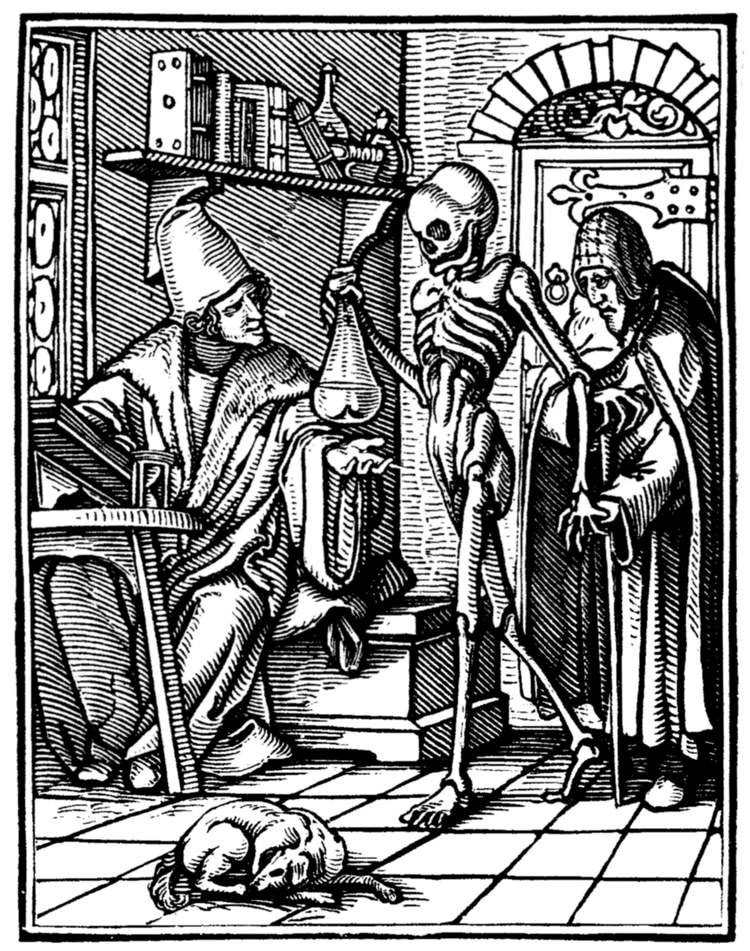
\includegraphics[width=0.51\textwidth]{assets/holbein-physician.jpg}
    \\
    \emph{The Physician}
    \\
    from Hans Holbein's \emph{Danse Macabre}
\end{figure}

\begin{center}
\parbox{200pt}{\lettrine[lines=3,slope=-2pt,nindent=-4pt]{\textcolor{SchoolColor}{T}}{his
thesis was typeset} using \LaTeX, originally developed by Leslie Lamport and
based on Donald Knuth's \TeX. The body text is set in 11 point Egenolff-Berner
Garamond, a revival of Claude Garamont's humanist typeface. The interactive
Python interpreter examples, and their graphic output, were handled by the
\emph{abjad-book} tool. }
\end{center}